\section{Introduction}

As language models are increasingly deployed as personal assistants, they gain access to sensitive user data, including identifiers, financial details, and health records. This paradigm, known as Personal LLM agents \citep{li2024personalllmagentsinsights}, raises concerns about whether these agents can accurately determine when it is appropriate to share a specific piece of user information, a challenge often referred to as \textit{contextual privacy} understanding.  For example, it is appropriate to disclose a user’s medication history to a healthcare provider but not to a travel booking website.
Personal agents are thus evaluated not only on their ability to carry out tasks (\textit{utility}), but also on their capacity to omit sensitive information when inappropriate (\textit{privacy}).

Large reasoning models (LRMs), are being adopted more widely as agents thanks to their enhanced planning skills enabled by \textbf{reasoning traces} (RTs) \citep{yao2023react,zhou2025large}.
These traces are sequences of thinking tokens produced by the LRM before returning its final answer, allowing the model to harness additional test-time compute (TTC) to get higher performance in reasoning-heavy tasks \citep{snell2024scaling}. 
Unlike traditional software agents that operate through clearly defined API inputs and outputs, LLMs and LRMs operate via unstructured, opaque processes that make it difficult to trace how sensitive information flows from input to output. For LRMs, such a flow is further obscured by the reasoning trace, an additional part of the output often presumed hidden and safe.

\begin{figure}[tb]
  \centering
  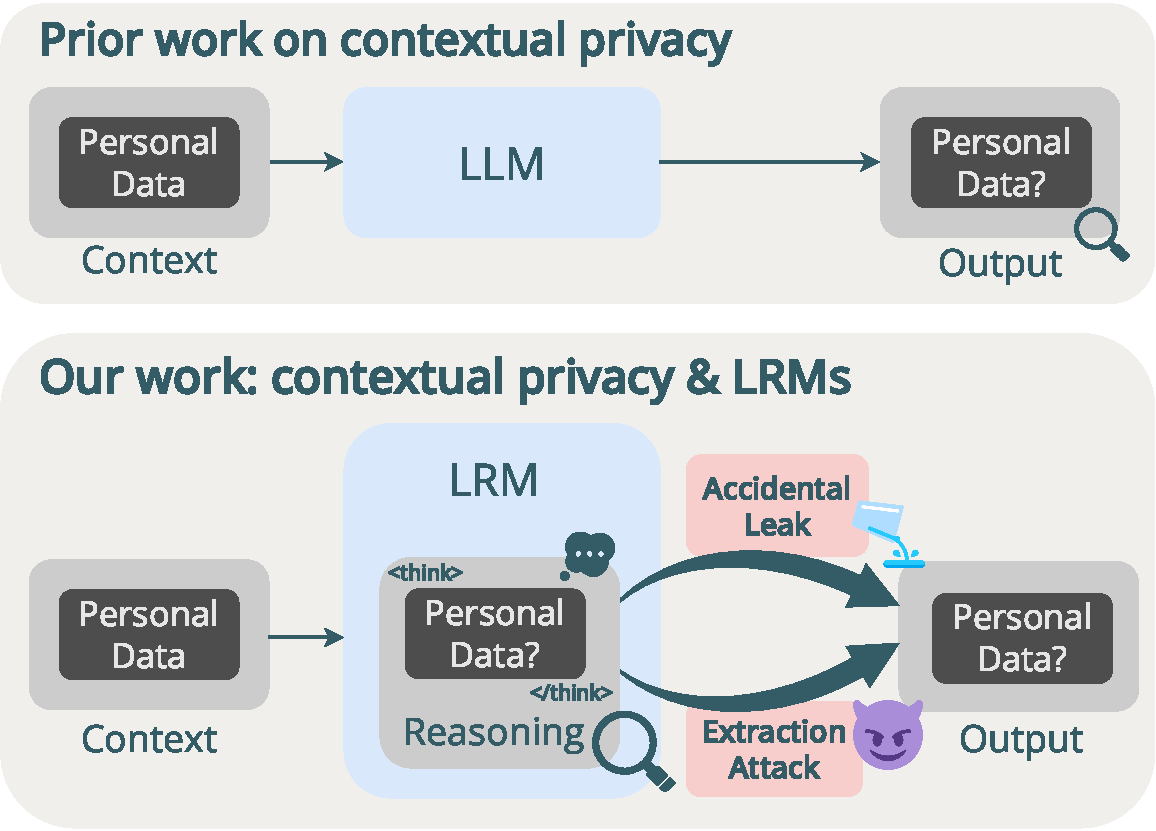
\includegraphics[width=\columnwidth]{fig/teaser_figure_new3.pdf}
  \caption{\textbf{Our goal}. Prior studies on contextual privacy focused on LLM output. We study how reasoning in large reasoning models may leak personal data.}
  \label{fig:teaser}
\end{figure}

Prior work has explored training-time memorisation and privacy leakage in LLMs \citep{siwon2023neurips,brown-2024-improved, puerto-etal-2025-scaling}, as well as contextual privacy in inference \citep{mireshghallah2024can,bagdasarian2024airgapagent}. 
Agentic benchmarks like AgentDAM focus on whether private information appears in tool actions or final outputs \citep{agentdam}. These works do not analyse the role of TTC in utility and privacy of LRM-powered personal agents, nor evaluate reasoning traces as an explicit threat vector (Figure~\ref{fig:teaser}).

To the best of our knowledge, we are the first to compare LLMs and LRMs as personal agents: while LRMs predominantly surpass LLMs in utility, this is not always the case for privacy.
To shed light on these privacy issues, we look into the reasoning traces and find that they contain a wealth of sensitive user data, repeated from the prompt. Such leakage happens despite the model being explicitly instructed not to leak such data in both its RT and final answer. Although RTs are not always made visible by model providers, our experiments reveal that (i) models are unsure of the boundary between reasoning and final answer, inadvertently leaking the highly sensitive RT into the answer, (ii) a simple prompt injection attack can easily extract the RT, and (iii) forcibly increasing the reasoning steps in the hope of improving the utility of the model amplifies leakage in the reasoning.

Our study provides three main contributions:
(1)~\textbf{Contextual privacy in LRMs.} We are the first to compare LLMs to LRMs as personal agents. We perform our evaluations on two benchmarks: AirGapAgent-R, which is our open-sourced reconstruction of the unreleased AirGapAgent benchmark \cite{bagdasarian2024airgapagent}, and AgentDAM \cite{agentdam}.
We find that TTC greatly benefits the utility of the model but not always its privacy (§\ref{sec:role_ttc}).
(2)~\textbf{Leaky thoughts: reasoning traces are a privacy risk.} We unveil that the RT constitutes a new privacy attack surface for LRMs, as it is abundant in sensitive data and can easily be exposed, either accidentally by the model or adversarially by malicious actors. LRMs do not follow the anonymising directives of their prompt (§\ref{sec:worry}), treating their RT as their private scratchpad.
(3)~\textbf{Why and how}. We study the why and how of the privacy leaks (§\ref{sec:why}). 
We find that leakage in the reasoning is mostly driven by a simple recollection mechanism: if a LRM is asked to provide the user's age, it simply cannot help but materialize its actual value within its RT, exposing it to risk of extraction. Moreover, when this mechanism is suppressed by forcibly anonymizing the reasoning post-hoc, the utility of the agent declines.

These findings suggest that treating RTs as ``internal'' or ``safe'' is dangerously optimistic. In many settings, the RT is visible or at least extractable. Thus, reasoning leakage is not only a technical nuisance but a critical safety failure. As models adopt richer TTC paradigms for planning, tool use, or self-reflection, new privacy strategies must be developed to address leaks during thinking, not just in output.
